%=== CHAPTER FIVE (5) ===
%=== Discussion ===

\chapter{Experimental Results and Discussion}
\label{cha:experiments}
\begin{spacing}{1.5}
\setlength{\parskip}{0.3in}

\section{Introduction}

Saysomething I am giving up on you..

\section{Test Metrics}

We use F1 Score and Accuracy as the test metrics.

Accuracy is given in \autoref{eq:acc}. The symbols in the equation means: TP for true positive, which is correctly predicted positive pixel number; TN for true negative, which is correctly predicted negative pixel number; FP for false positive, which is number of positive pixels being predicted as negative; FN for false negative, which is number of negative pixels being predicted as positive. \autoref{fig:testtp} gives clearer interpretation.

\begin{equation}
\label{eq:acc}
    Accuracy=\frac{TP+TN}{TP+TN+FP+FN}=\frac{TP+TN}{All}
\end{equation}

\begin{figure}[ht]
\centering
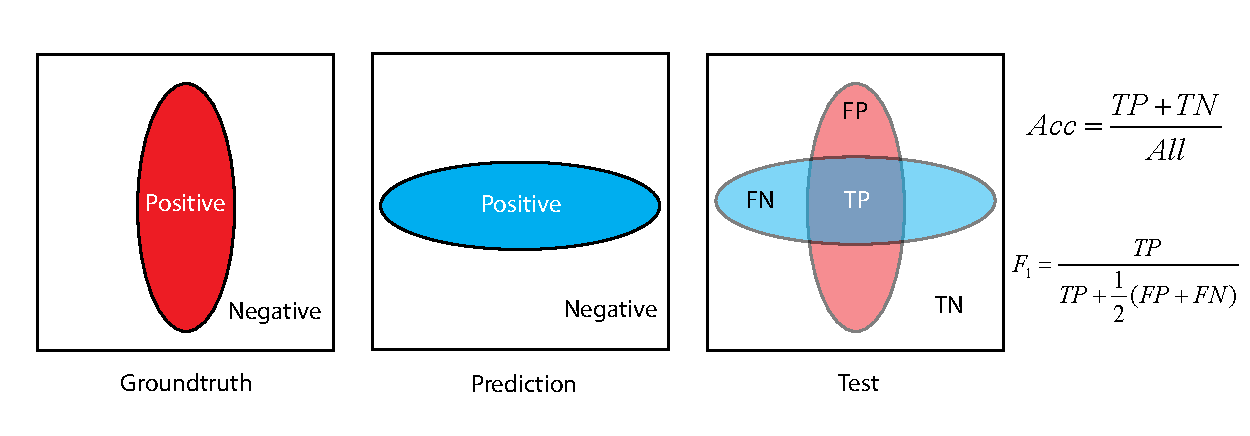
\includegraphics[width=0.99\textwidth, fbox]{Chapter5/testtp.pdf}
\caption{TP, TN, FP and FN in Binary Classification}
\label{fig:testtp} 
\end{figure}

The standard $F_1$ score is given in \autoref{eq:f1score}

\begin{equation}
\label{eq:f1score}
    F_1=\frac{TP}{TP+\frac{1}{2}(FP+FN)}
\end{equation}

Specially, when there's no positive pixel in ground truth and the predicted feature map are all-negative, $F_1$ score calculated by \autoref{eq:f1score} is zero. However, in this case, all the pixels are predicted precisely. So we set $F_1$ score as $1$ in this special case.

Besides, we use the metric described in Section 5.3, VPGNet~\cite{lee2017vpgnet} to calculate the $F_1$ score: 1) calculate the minimum distance between grids' center and sampled lane points. 2) If the minimum distance is smaller then a boundary value $R$, the sampled lane points are marked as positive. This is for complying with the output size and the $8 \times 8$ grid size in VPGNet. The python code of $F_1$ score calculation are given in \autoref{apx:testmetrics}.

\section{Multi-class Visualization Tool}

\begin{figure}[!p]
    \centering
    \begin{subfigure}[b]{0.49\textwidth}
        \centering
        \includegraphics[width=2.7in, fbox]{Chapter5/Picture1.jpg}
        \caption{Picture 1}
    \end{subfigure}%
    ~
    \begin{subfigure}[b]{0.49\textwidth}
        \centering
        \includegraphics[width=2.7in, fbox]{Chapter5/Picture1an.jpg}
        \caption{Annotated Picture 1, $\alpha$=0.6}
    \end{subfigure}
    \\
    \begin{subfigure}[b]{0.49\textwidth}
        \centering
        \includegraphics[width=2.7in, fbox]{Chapter5/Picture2.jpg}
        \caption{Picture 2}
    \end{subfigure}%
    ~
    \begin{subfigure}[b]{0.49\textwidth}
        \centering
        \includegraphics[width=2.7in, fbox]{Chapter5/Picture2an.jpg}
        \caption{Annotated Picture 2, $\alpha=0.8$}
    \end{subfigure}
    \\
    \begin{subfigure}[b]{0.49\textwidth}
        \centering
        \includegraphics[width=2.7in, fbox]{Chapter5/Picture3.jpg}
        \caption{Picture 3}
    \end{subfigure}%
    ~
    \begin{subfigure}[b]{0.49\textwidth}
        \centering
        \includegraphics[width=2.7in, fbox]{Chapter5/Picture3an.jpg}
        \caption{Annotated Picture 3, $\alpha=1$}
    \end{subfigure}
    \caption{Annotation with Different Colors and Transparency}
    \label{fig:annotation}
\end{figure}


In our work, we developed an automatic annotation tool for visualization the lane detection result. It can show different classes in different color. As shown in \autoref{fig:annotation}, different classes are given colors that are easy to distinguish from each other, and the transparency of the annotation label can be adjusted by factor $\alpha$. This tool can also be used in other multi-label classification tasks, so the code are included in \autoref{apx:extraction}.

\section{Multi-class Performance}


\begin{figure}[ht]
    \centering
    \begin{subfigure}[b]{0.99\textwidth}
        \centering
        \includegraphics[width=0.98\textwidth, fbox]{Chapter5/testloss20000.pdf}
        \caption{Loss of $20,000$ Epoch}
    \end{subfigure}
    \\
    \begin{subfigure}[b]{0.99\textwidth}
        \centering
        \includegraphics[width=0.98\textwidth, fbox]{Chapter5/testloss100000.pdf}
        \caption{Loss of $100,000$ Epoch}
    \end{subfigure}
    \caption{Loss of different Epochs in CAFFE}
    \label{fig:testloss}
\end{figure}


First, we conducted experiments on CAFFE with different epochs. The training result are shown in \autoref{tab:cafferesult}. The raw data line is accompanied with a regression curved line to show the tendency, and for clearer show the tend of decreasing, the $Y$-axis is set as Log scale.

\begin{table}[ht]
\centering
\caption{Training Result on CAFFE}
\label{tab:cafferesult}
\begin{tabular}{@{}cccc@{}}
\toprule
\textbf{Epochs} & \textbf{Combined Loss} & \textbf{$Acc_{mask}$} & \textbf{$Acc_{class}$} \\ \midrule
1,000 & 3.73851 & 92.1165\% & 91.6981\% \\
10,000 & 2.7172 & 95.4574\% & 93.5048\% \\
20,000 & 2.53835 & 95.714\% & 93.7822\% \\
40,000 & 2.32726 & 97.37\% & 96.2012\% \\
70,000 & 2.24239 & 97.6137\% & 96.5076\% \\
97,400 & 1.99095 & \textcolor{red}{97.7479\%} & \textcolor{red}{97.1909\%} \\ \bottomrule
\end{tabular}
\end{table}

To avoid over fitting, we plot the $20,000$ epochs and $100,000$ epochs experiment loss as in \autoref{fig:testloss}, with a regression curve and Y-axis set as log scale. As can be seen, the loss is decreasing rapidly and converge at around $2.12$. In our experiment, because the loss decreasing rate for different branches are different, as shown in \autoref{fig:testlossbranch}, we set $3:1:1$ weight for grid, masking and pixel classification tasks. The combined loss is shown in \autoref{eq:combineloss}

\begin{equation}
\label{eq:combineloss}
    Loss_{comb}=w_1*{Loss_{grid}}+w_2*{Loss_{masking}}+w_3*{Loss_{cls}}
\end{equation}

in which $w_1=\frac{3}{3+1+1}=0.6$, $w_2=w_3=\frac{1}{3+1+1}=0.2$.

\begin{figure}[ht]
\centering
\includegraphics[width=0.99\textwidth, fbox]{Chapter5/testlossbranch.pdf}
\caption{Test Loss in Three Branches Decrease with Different Rate}
\label{fig:testlossbranch} 
\end{figure}

The accuracy of the multi-label pixel classification task and masking task are shown in \autoref{fig:testacc}. Notice that the Y-axis range is $(0,1)$ and is in Logit scale, because they are close to each other when close to $1$.

\begin{figure}[ht]
\centering
\includegraphics[width=0.99\textwidth, fbox]{Chapter5/testacc.pdf}
\caption{Test Accuracy Curve in Logit Scale $(0,1)$}
\label{fig:testacc} 
\end{figure}

\section{Rainy Condition}

Select severe pictures dedicated.

\section{Post-processing}

\subsection{Selection of Confidential Threshold}

Compare of Threshold results

\subsection{Contour}


\section{Concluding Remarks}

something conclusion.

%=== END OF CHAPTER FIVE ===
\end{spacing}
\newpage
